%%%%%%%%%%%%%%%%%%%%%%%%%%%%%%%%%%%%%%%%%%%%%%%%%%%%%%%%%%%%%%%%%%%%%%%%%%%
%% This file is part of the book
%%
%% Algorithmic Graph Theory
%% http://code.google.com/p/graph-theory-algorithms-book/
%%
%% Copyright (C) 2009, 2010, 2011 Minh Van Nguyen <nguyenminh2@gmail.com>
%%
%% See the file COPYING for copying conditions.
%%%%%%%%%%%%%%%%%%%%%%%%%%%%%%%%%%%%%%%%%%%%%%%%%%%%%%%%%%%%%%%%%%%%%%%%%%%

\documentclass{article}

\usepackage{tikz}
\usetikzlibrary{external}
\usetikzlibrary{trees}
\tikzexternalize{Fibonacci-tree-height}

\begin{document}

\begin{figure}
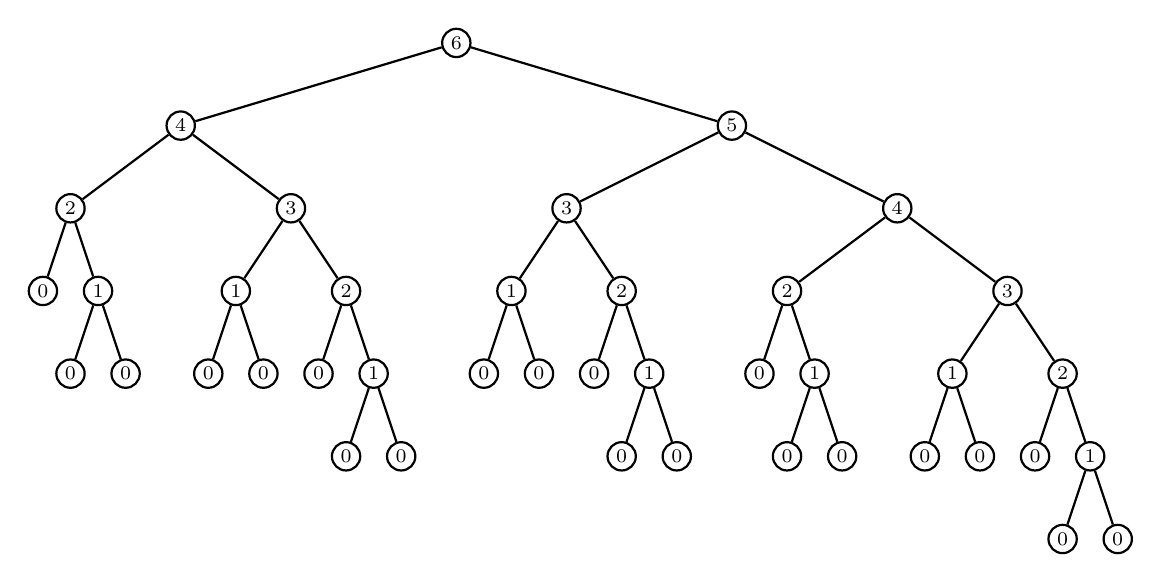
\begin{tikzpicture}
[-,thick,%
  every node/.style={shape=circle,inner sep=1.5pt,draw,thick},%
  scale=0.7]
\scriptsize
\node {$6$}
  [sibling distance=10cm]
  child {node {$4$}
    [sibling distance=4cm]
    child {node {$2$}
      [sibling distance=1cm]
      child {node {$0$}}
      child {node {$1$}
        child {node {$0$}}
        child {node {$0$}}
      }
    }
    child {node {$3$}
      [sibling distance=2cm]
      child {node {$1$}
        [sibling distance=1cm]
        child {node {$0$}}
        child {node {$0$}}
      }
      child {node {$2$}
        [sibling distance=1cm]
        child {node {$0$}}
        child {node {$1$}
          child {node {$0$}}
          child {node {$0$}}
        }
      }
    }
  }
  child {node {$5$}
    [sibling distance=6cm]
    child {node {$3$}
      [sibling distance=2cm]
      child {node {$1$}
        [sibling distance=1cm]
        child {node {$0$}}
        child {node {$0$}}
      }
      child {node {$2$}
        [sibling distance=1cm]
        child {node {$0$}}
        child {node {$1$}
          child {node {$0$}}
          child {node {$0$}}
        }
      }
    }
    child {node {$4$}
      [sibling distance=4cm]
      child {node {$2$}
        [sibling distance=1cm]
        child {node {$0$}}
        child {node {$1$}
          child {node {$0$}}
          child {node {$0$}}
        }
      }
      child {node {$3$}
        [sibling distance=2cm]
        child {node {$1$}
          [sibling distance=1cm]
          child {node {$0$}}
          child {node {$0$}}
        }
        child {node {$2$}
          [sibling distance=1cm]
          child {node {$0$}}
          child {node {$1$}
            child {node {$0$}}
            child {node {$0$}}
          }
        }
      }
    }
  };
\end{tikzpicture}
\end{figure}

\end{document}
